
\documentclass[12pt]{article}

\usepackage{scicite}
\usepackage{times}
\usepackage{graphicx}
\usepackage{hyperref}
\usepackage{enumitem}
\usepackage{amsmath}

\topmargin -1.5cm
\oddsidemargin 0.0cm
\textwidth 16cm 
\textheight 23.5cm
\footskip 1.0cm

\newenvironment{sciabstract}{%
\begin{quote} \bf}
{\end{quote}} 

\newcounter{lastnote}
\newenvironment{scilastnote}{%
  \setcounter{lastnote}{\value{enumiv}}%
  \addtocounter{lastnote}{+1}%
  \begin{list}%
  {\arabic{lastnote}.}
  {\setlength{\leftmargin}{.22in}}
  {\setlength{\labelsep}{.5em}}
}
{\end{list}}

\title{Assignment 2} 

\author
{Filipe Pires [85122], Joao Alegria [85048]\\
\\
Information Retrieval\\
\normalsize{Department of Electronics, Telecommunications and Informatics}\\
\normalsize{University of Aveiro}\\
} 

\date{\today{}}

%%%%%%%%%%%%%%%%% END OF PREAMBLE %%%%%%%%%%%%%%%%

\begin{document} 
\baselineskip18pt
\maketitle 

\section*{Introduction}

This report was written as a follow-up work of the delivery of the first 
assignment for the discipline of 'Information Retrieval' and describes both
the updates made on the initial solution and the development of new features 
related to the indexing of text corpus.

We include the updates done on each class developed and on the respective
methods, as well as the redesign of our class diagram.
We also provide the instructions on how to run our code.

An explanation on the implementation of the SPIMI approach for the indexing
process that considers memory limitations is presented in this report.
Changes to the output file (the actual index) format are also explained.

Along with the description of the solution, we also answer to a few questions
proposed for the assignment \cite{assign2}.
All code and documentation is present in our public GitHub project at 
\url{https://github.com/joao-alegria/RI}. 

\newpage
\section*{1. Updates to Assignment 1}

Once concluded the period of time dedicated for the development of the work 
proposed for the first assignment, some mistakes on our delivery were
detected and we found that their solution, although simple, was important to
be presented in this next assignment.

In point d) of the 4th task of assignment 1, it was asked for us to present
the ten terms with highest document frequency according to the index produced
by our program using both tokenizer implementations.
Our mistake was that we presented the ten terms with highest collection 
frequency. To make up for this error, we decided to present here the ten terms
with highest document frequency, as well as those with highest collection 
frequency and those with highest term frequency.
The difference between these 3 statistical properties are presented below:

\begin{itemize}[leftmargin=*]
\setlength\itemsep{-0.3em}
\item Document Frequency - the number of documents in a collection where 
a given token occurs.
\item Term Frequency - the number of occurrences of a given token in a 
document.
\item Collection Frequency - the total number of occurrences of a given 
token in the collection.
\end{itemize}

The 10 terms with highest document frequency (for both tokenizers) are the 
following:

\begingroup
\addtolength\leftmargini{-0.4in}
\addtolength\baselineskip{-0.05in}
\begin{quote}
\begin{verbatim}
Simple:
Terms: 'and' (1739514), 'the' (1589467), 'with' (598916), 
'for' (585442), 'from' (229502), 'patients' (226388), 
'human' (211802), 'cell' (171278), 'cells' (167779), 
'study' (167384).

Complex:
Terms: 'cell' (323874), 'patient' (284668), 'effect' (279130),
'human' (226069), 'studi' (215412), 'activ' (192730),
'use' (176649), 'protein' (175199), 'rat' (171824),
'diseas' (165580).
\end{verbatim}
\end{quote}
\endgroup

The 10 terms with highest term frequency (for both tokenizers) are the 
following:

\begingroup
\addtolength\leftmargini{-0.4in}
\addtolength\baselineskip{-0.05in}
\begin{quote}
\begin{verbatim}
Simple:
Terms: ['the'] (14), ['alpha','ucdeq'] (12), ['mcm'] (11),
['and','eta','mcma','nov','nvheq','sorbitan','tky'] (10).

Complex:
Terms: ['alpha'] (11), ['eta','nov','sarcosin','sorbitan'] (10),
['edta','failur','kinas','manp'] (9), ['beta','buttiauxella',
'hla','mycoplasma','placent','pseudomona', 'silic','subsp',
'tick','val'] (8).
\end{verbatim}
\end{quote}
\endgroup

\newpage
The 10 terms with highest collection frequency (for both tokenizers) are the 
following:

\begingroup
\addtolength\leftmargini{-0.4in}
\addtolength\baselineskip{-0.05in}
\begin{quote}
\begin{verbatim}
Simple:
Terms: 'and'(2044099), 'the'(2033707), 'with'(633062), 
'for'(608296), 'from'(234101), 'patients'(228824),
'human'(217457), 'cell'(184034), 'cells'(174998),
'study'(170588)

Complex:
Terms: 'cell'(359036), 'patient'(289130), 'effect'(281633),
'human'(232049), 'studi'(219451), 'activ'(202904),
'protein'(188952), 'use'(178166), 'rat'(173397),
'diseas'(169893)
\end{verbatim}
\end{quote}
\endgroup

Let us now take a look at the updates made for the purpose of this second 
assignment.

The first update we made to our code was on the content of the index files 
produced by our indexer. Initially it would write to a text file a token
per line followed by a comma (',') and all document IDs of the documents that
contained the respective token, paired with the respective frequency (with
a ':' between each docID and frequency value).
For this assignment, we altered the format in order be possible to store the position
of each occurrence and the term frequency weight (tfw) and inverse document 
frequency (idf) of each term, following the given format:

\begingroup
\addtolength\leftmargini{-0.4in}
\begin{quote}
\begin{verbatim}
token:idf, docID:tfw:pos1,pos2,...; docID:tfw:...; ...
\end{verbatim}
\end{quote}
\endgroup

Actually, we implemented this in such way that it is possible for the user
to choose from 4 different combinations of output formats, varying the 
presentation of either the frequency or the weight and the presentation or
not of the positions of the terms in each document.
Although this was not specifically asked in the assignment instructions,
it answers its requirements and gives the user a wider range of usage 
alternatives.

Regarding the structure of our abstract classes, a few changes had to be
considered to better face the challenges of the second assignment.
These, however, were not very relevant in terms of difficulty or time
consumption.

The capacity of regulating the amount of memory used during the program's
execution was a more complex task, with several aspects that required close
attention. Our work on the implementation of a SPIMI approach is explained
in detail further ahead, but it is good to mention that a few updates to 
the {\it main()\/} function had to be made in order for this and all other 
changes to be supported by the new version of the program.
Still on the updates to the initial phases of the program execution, it is
important to mention that we altered the way we process the arguments passed
to the scripts when running them. The changes were made to employ the standard
form of dealing with script parameters, with the help of the \texttt{getopt}
Python library \cite{getopt}.

\section*{2. Architecture \& Memory Usage}

The remaining of the report supposes that the reader has knowledge about what
was presented on the first delivery. 
We will only explain the structure of new components not yet seen by the reader 
and the updates made on the class diagram.

In this chapter we also get into deeper detail on how is memory usage
considered, as well as on how are the new attributes such as the term weights 
calculated and stored.
Figure \ref{fig:classdiagram} shows the new class diagram, with a considerable
increase in complexity compared to the initial version.

\begin{figure}[h!]
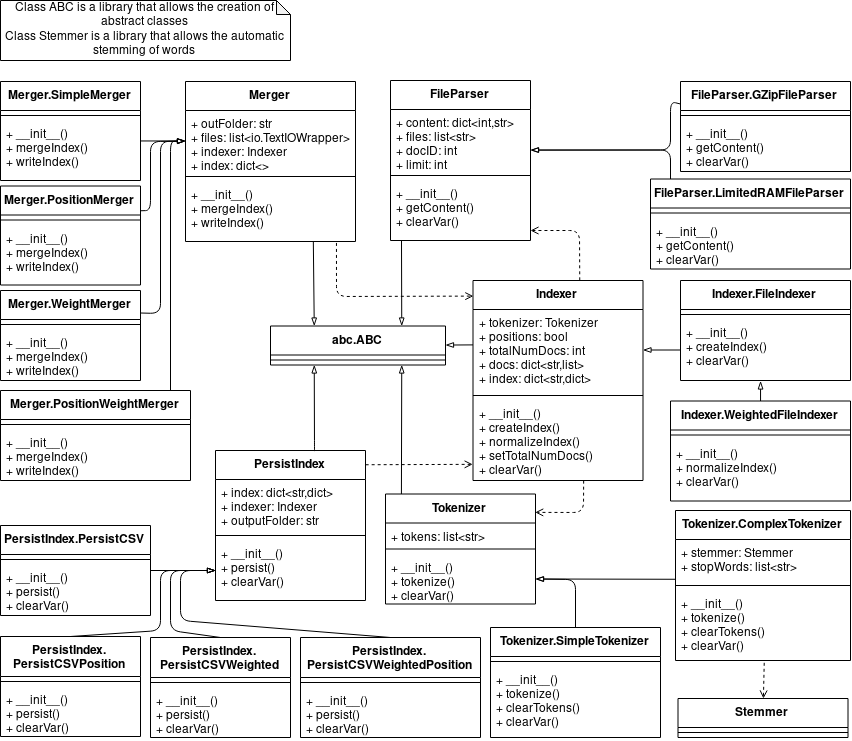
\includegraphics[width=\linewidth]{ClassDiagram_assign2.png}
\caption{Program's class diagram.}
\label{fig:classdiagram}
\end{figure}

First of all, we have the new class derived from \texttt{FileParser} with the
name \texttt{LimitedRAM} \texttt{FileParser}. This class does the same as its 
"sister" \texttt{GZipFileParser}, except that \textit{getContent()} is now 
called 1 time per document and returns the information relative to that 
document only. 
Although this makes the reading process slower, it allowes the user to have a 
improved control over the RAM consumption.

The \texttt{WeightedFileIndexer} is a new class derived from our 
\texttt{FileIndexer}.
This class inherits the method \textit{createIndex()} from our previous 
implementation and makes use of the method \textit{normalizeIndex()} to calculate 
the term frequencies. 
We call it a normalization as it is a transformation of the produced index to
standardize its values according to a set of rules.
We calculate the term frequencies following the logarithmic formula variant and 
the process of normalization is based on the cosine formula variant, both 
presented bellow.

\begin{equation*}
tf_{t,d} = 1 + log(tf_{t,d}) \>\>\>\>\>
\>\>\>\>\> W = \frac{1}{\sqrt{w_1^2 + w_2^2 + ... + w_M^2}}
\end{equation*}

The \texttt{Tokenizer} implementations were the only classes that suffered no
changes nor recieved no new subclasses. 
Our solution served perfectly for the tokenization process whether the program 
is executed with a memory limitation or not.

For the \texttt{PersistIndex} class, we developed 3 new classes derived from 
it - one for each new output format. 
Following are small portions of indexes generated by our solution in the formats
supported by the program, for analysis purposes(all with the complex tokenizer).

Simple Output(in output/complexSample.txt):
\newline ...
\newline acetyl,133:1
\newline acid,54:1,55:1,65:1,72:1,81:1,86:1,91:1,104:1,112:1,116:1,126:1,159:1,171:1
\newline ...
\newline

Positions Output(in output/complexP):
\newline ...
\newline acetyl;133:1:4
\newline acid;54:1:10;55:1:7;65:1:4;72:1:4;81:1:2;86:1:8;91:1:4;104:1:10;112:1:4;116:1:7;126:1:8;159:1:4;171:1:7
\newline ...
\newline

Weights Output(in output/complexW):
\newline ...
\newline acetyl:2.35;133:1.0
\newline acid:1.24;54:0.28;55:0.28;65:0.28;72:0.28;81:0.28;86:0.28;91:0.28;104:0.28;112:0.28;
\newline 116:0.28;126:0.28;159:0.28;171:0.28
\newline ...
\newline

\newpage
Weights+Positions Output(in output/complexWP):
\newline ...
\newline acetyl:2.35;133:1.0:4
\newline acid:1.24;54:0.28:10;55:0.28:7;65:0.28:4;72:0.28:4;81:0.28:2;86:0.28:8;91:0.28:4;
\newline 104:0.28:10;112:0.28:4;116:0.28:7;126:0.28:8;159:0.28:4;171:0.28:7
\newline ...
\newline

We now proceed to explaining how was the memory considered in this second 
assignment and, more specifically, what is the SPIMI strategy already 
mentioned in this document.
SPIMI stands for Single-Pass In-Memory Indexing, and its key ideas are 
that several pseudo-indexes (index approximations) are generated, one per 
block of information (where, in our case, a block represents the amount 
of information capable of being stored in memory alone), accumulating 
postings (details about each term) in postings lists as they occur. 
Then, these block-indexes are merged with a n-way merge, for efficiency 
purposes, into a unique index.
This final index, however, is stored in one or more output files, 
according to the memory restrictions applied to the program.

Our solution has the following execution flow: while there is still memory 
available, the program parses one document, tokenizes it and adds it to an
internal index; if the memory limit is reached, this internal index is then 
normalized and persisted to disk according to the chosen format, and finally 
the memory is cleared and the cicle continues.
Once the entire corpus has been processed, if needed, the merger is created 
and the n-way merge is executed to produce the final index. 
The memory used by the process responsible for the program's execution is 
assured never to exceed the memory limitation applied by the user.

\newpage
\section*{3. Index Merging}

We have not yet talked about the \texttt{Merger} class, although it has 
already been mentioned that a merging process takes place in this second 
assignment.
This chapter is dedicated to this new module of our solution and the 
decisions made during its implementation.

How exactly does the n-way merge work? 
The most straightforward solution would be to merge index files in pairs, 
by directly comparing each line and merging each into one. This process 
would repeat until all files were reduced to one.
The problem with this alternative is that, after each pair merging process, 
the newly created index file will have to be processed again - this adds a 
redundancy that severly slows the execution.
This is where the n-way merging fits in.
To solve the redundancy problem, we iterate over all index files (n means 
the number of files) simultaneously. 
This way, we guarantee that each line is only processed once.

The way we implemented the n-way merge works as follows.
With the aid of a temporary array, we store the latest line of each index 
file, one at a time; when this occurs for all files, we calculate the 
minimum term by finding the minimum (alphabetically) of the auxiliary array. 
If the minimum term appears more than once in the array, the merging of the 
respective postings lists happens, followed by storing those values in an 
internal (in-memory) index.
The positions in the temporary array where the merging of the term occurred
are replaced by an empty value.
New lines are only inserted where the array contains these empty values and 
they are fetched from the respective index file.
Now the process repeats itself, constantly merging the terms that occur in 
more than one index file, and storing the merged term in the internal index.
Once this in-memory index reaches a point where there is no more free memory 
available, its content is then written to disk and the memory is freed so 
that the process can continue with the remaining terms.

\newpage
\section*{4. Discussion}

To test the capabilities of the developed software, we indexed the same
2 large compressed files used on the previous deliver, with the names 
\texttt{2004\_TREC\_ASCII\_MEDLINE\_1.gz} and 
\texttt{2004\_TREC\_ASCII\_MEDLINE\_2.gz}.
Their structure, as collections (corpus) of documents, remained the same.
In this chapter we discuss our implementation's efficiency over these 
files according to the following measures:

a) What is the total indexing time and final index size on disk?

b) What is the maximum amount of memory used during indexing?

Although running the program works very similarly to the previous version, we
present here the updated format.
The file \texttt{CreateIndex.py} serves as the pipeline creator and is ther command to be executed in order to 
indexing all documents passed as arguments, and it has the following execution options:

\begingroup
\addtolength\leftmargini{-0.4in}
\addtolength\baselineskip{-0.05in}
\begin{quote}
\begin{verbatim}
$ python3 CreateIndex.py [-h] [-p] [-w] [-o outputFolder] 
  [-l limit] [-t tokenizer] [-r limitRAM] inputFolder
\end{verbatim}
\end{quote}
\endgroup

Here, \texttt{-h} is the option that presents the manual for the command usage.
Options \texttt{-p} and \texttt{-w}, if present, tell the program to process the
positions and weights of the terms in the index, respectively.
Options \texttt{-o} and \texttt{-l} allow the definition of the output folder's 
name and of the limit for the number of lines to be processed in each input file.
Option \texttt{-t} makes possible for the user to choose the type of tokenizer
to be used, and the alternatives are: 'simple' for the use of the 
\texttt{SimpleTokenizer} class, and 'complex' for the \texttt{ComplexTokenizer} class.
Option \texttt{-r} allows the user to define the maximum amount of memory that can
be used by the process running the program.
The previous arguments are all optional and the actual values for these arguments
must appear right after the respective options.
The final argument of the command must be the name of the folder that contains the
files to be indexed. This argument was changed since last assignment as we considered
more user-friendly to identify the target folder rather than each one of the input files
(this is more noticeable as the number of files increases). Other argument that changed
was the output option, transitioning from file name to folder name since now it's possible
to create more than one file as the output index and to maintain a user-friendly application we decided
to make this adjustment.

The final version of our solution was executed according to the following format,
as requested on the question 2 (the input folder contained the compressed
files previously mentioned):

\begingroup
\addtolength\leftmargini{-0.4in}
\addtolength\baselineskip{-0.05in}
\begin{quote}
\begin{verbatim}
$ command time -v python3 CreateIndex.py -o ../index -w 
  -t complex -r 0.5 ../input
\end{verbatim}
\end{quote}
\endgroup

The results are here presented. The total indexing time, given by the command
"command time -v" was of 60 minutes . 
The final index size on disk is calculated by summing the size on disk of the 
various sub-indexes generated by the merger. 
The result was of 491.4 Mb .

The maximum amount of memory used during indexing was also given by the 
"command time -v" command and had a value of 462 Mb , meaning that
the memory limit given of 500Mb was indeed not surpassed.

In relation to the question 3, the final results were obtained by running the 
following command:

\begingroup
\addtolength\leftmargini{-0.4in}
\addtolength\baselineskip{-0.05in}
\begin{quote}
\begin{verbatim}
$ command time -v python3 CreateIndex.py -o ../index -wp 
  -t complex -r 0.5 ../input
\end{verbatim}
\end{quote}
\endgroup

The total indexing time was of 61 minutes. The final index size on disk was  577.3 Mb .
Finnaly the maximum amount of memory used during indexing was 487 Mb.

Taking a closer look at the results, the first fact that takes our attention is the
execution time.
When we compare it to the initial solution (of the first assignment), we see an
increase in time of 500 \%.
This is explained by the fact that, not only the reading process becomes slower
as the number of accesses done to the input files are increased, but also the 
number of writes to disk also increase as well as the number of files we write to.
All these I/O interactions, i.e. accesses to disk, are very time consuming and 
are a good example of the well-known bottleneck problem of high resource-demanding tasks.
The advantage of these interactions lies on the reduction of other resource usages - 
more specifically, of RAM usage. 
By indexing large files with this method, we guarantee that the program can process
corpus that far exceed the hardware resources available.
The user now gains power to balance resource usage according to his / her needs and
available hardware.

The second observation we find important to refer regards the final index storage 
strategy. We decided to store the outcome in several partial index files since we
took into account that, in the future, the aim will be to retrieve information from
them through queries and so these partial index files will allow for a faster retrieval
of results.

\newpage
\section*{Conclusions}

After completing the assignment, we drew a few conclusions regarding our
solutions and the whole concept of memory management and its balancing with
good efficiency.

The biggest challenge we faced was definetly the merging process.
As we wished to come up with a solution of our own, rather than using external code or 
libraries, the planning and execution took a considerable amount of time and effort.
In addition, testing was also not very much straightforward, as the results needed to
be manually checked.
The delivered code, although time consuming during its execution, ensures that no term
is lost, no attribute wrongly calculated and the results are exactly the same compared
to the outcome of the execution without memory limitation (i.e. without the merging of
intermediate indexes).

From this assignment, we take the importance of being able to control the tradeoff 
between indexing time and memory usage.
Although execution times greatly increases once memory restrictions are considered, we
saw a great value in being able to constrain the resources consumed by the process 
in order to allow for the operating system to still offer sufficient memory for other
tasks.

When it comes to teamwork, we follow a balanced work distribution, usually dedicating
the time for the assignment in compatible schedules. This helps keeping up-to-date with 
what each is doing and speeds up problem solving. 
% For this assignment, due to external factors, the impact weight of each team element
% differs a bit, with an estimated effort distribution of 60\% to Joao Alegria and 40\%
% to Filipe Pires.

\begin{thebibliography}{9}
  \bibliographystyle{Science}

  \bibitem{assign2}
    S. Matos,
    \textit{IR: Assignment 2},
    University of Aveiro,
    2019/20.
  \bibitem{getopt}
    GetOpt Library - C-Style Parser for Command Line Options,
    Python.org
    \textit{https://docs.python.org/2/library/getopt.html},
    (visited in 25/10/2019)
  
\end{thebibliography}

\clearpage

\end{document}




















